\chapter{Results}\label{section:results}

    Here we present the results from our two different experiments.

    We compare the results of our code-prose experiment to the original study~\cite{floyd_decoding_2017} and the replication study~\cite{fucci_replication_2019}, and investigate the results from our naturalistic device use experiment to see if results generalize to other types of device activity.

    \todo[inline]{Update with final values}

    \section{Code vs prose task}

        % FIXME: Fucci uses the median, should we too?
        Our top-performing classifier yields a LORO-CV mean BAC score of: $0.614 \pm 0.089$ (mean $\pm$ std).
        \todo[inline]{Markus: Mätetalet behöver introduceras i Kapitel 3 så att läsaren förstår innebörden här.}

        The following is the performance statistics for our model trained on \SI{5}{\second} windows. It is trained on all subjects except one, which is used in testing:

        \begin{verbatim}
        INFO: {
            'precision': 0.7473868367437329, 
            'recall': 0.696405129166862, 
            'fbeta': 0.6703482474923927, 
            'support': array([308, 277]), 
            'bac': 0.696405129166862, 
            'confusion_matrix': array([[141, 167], [ 18, 259]])
        }
        \end{verbatim}
        \todo[inline]{Markus: Nya mätetal här också. Det är ok att förklara vad de betyder här. Tolkningarna av resultaten kan vi fortfarande spara till nästa kapitel.}

        \todo[inline]{Markus: Vilken modell är det som gäller nu? Och vilka features och clearning och sånt bygger den på? Kanske avsluta kapitel 3 med att tydligt presentera vad som används i experimenten?}
        The following are the performance statistics for our model on the epoch-level. We achieve epoch-level classification by training on \SI{5}{\second} windows which are aggregated into epochs by taking the mean of the prediction probabilities. The same subject selection as the previous statistics is used:

        \todo[inline]{Use performance statistics from LORO-CV, not from single-subject validation}

        \begin{verbatim}
        INFO: {
            'precision': 0.8541666666666667, 
            'recall': 0.7666666666666666, 
            'fbeta': 0.7624602332979852, 
            'support': array([15, 17]), 
            'bac': 0.7666666666666666, 
            'confusion_matrix': array([[ 8,  7], [ 0, 17]])
        }
        \end{verbatim}

        \todo[inline]{Use LORO instead of testing subject}
        \begin{table}
            \begin{center}
                \begin{tabular}{lcc}
                  \toprule
                  & Epoch-level (subject \#6) & Window-level (subject \#6) \\ \midrule
                  Precision & 85.4\% & 74.7\% \\
                  Recall & 76.7\% & 69.6\% \\
                  BAC & 76.7\% & 69.6\% \\
                  \bottomrule
                  
                \end{tabular}
                \caption{Performance statistics of our models trained on all subjects except subject number \#6 which is used for testing}\label{fig:stats}
            \end{center}
        \end{table}

        %\begin{figure}[h]
        \begin{sidewaysfigure}
        \centering
        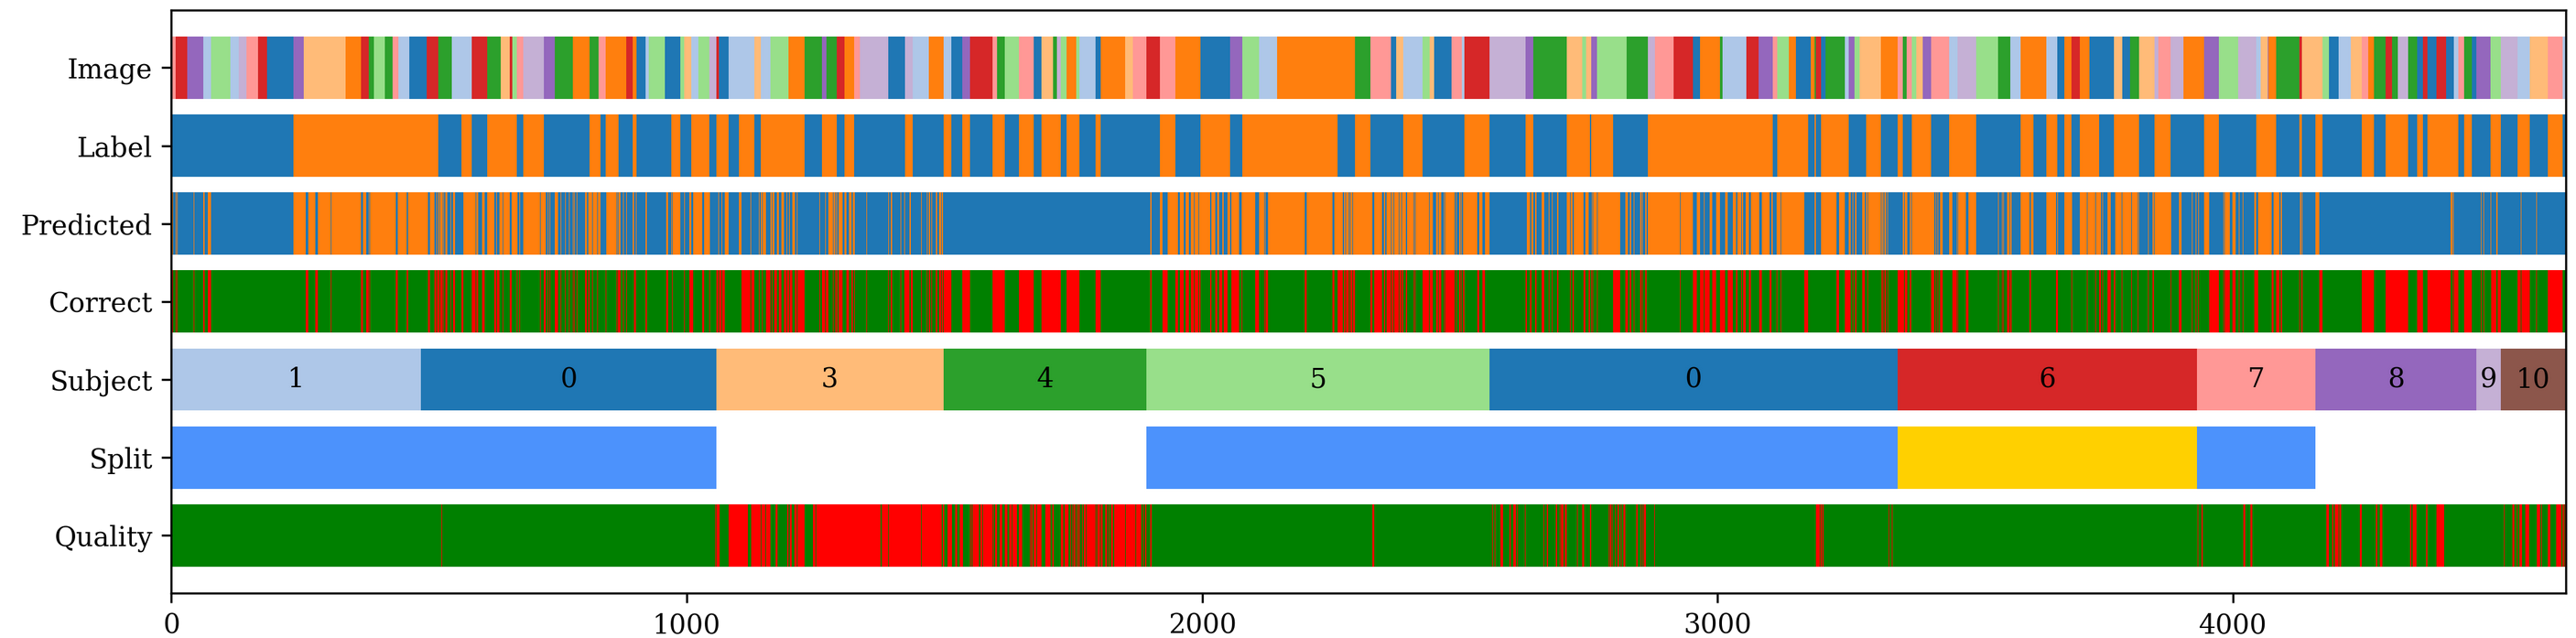
\includegraphics[width=24cm]{img/timebars.png}
        \caption{Visualization of the labeled data, the predicted class, the subject, the training and testing split, and a measure of signal quality. The x-axis is the window index, sorted by acquisition time.}\label{fig:timebars}
        \end{sidewaysfigure}
        %\end{figure}

        Our classifier performance is\ldots

        \begin{figure}[h]
        \centering
        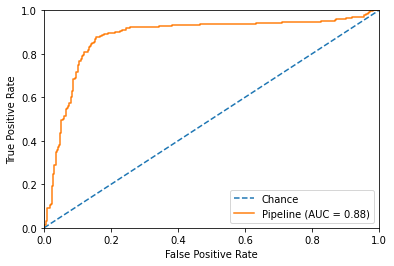
\includegraphics[width=12cm]{img/roccurve.png}
        \caption{Receiver operating characteristic (ROC) curve.}\label{fig:roc}
        \end{figure}
        \todo[inline]{Update with higher-res image}

        Compared to previous studies, we achieve a moderate improvement over the EEG-only classifier trained in Fucci et al., and achieve a similar performance to the fMRI study by Floyd et al. (seen in Table~\ref{table:compare-results}).

        \begin{table}
            \begin{center}
                \begin{tabular}{lccc}
                    \toprule
                    & \textbf{This study} & \textbf{Fucci et al.} & \textbf{Floyd et al.} \\
                    \midrule
                    Overall & 0.77 & 0.66 & 0.79 \\
                    Code & x & x & x \\
                    Prose & x & x & x \\
                    \bottomrule
                \end{tabular}
                \caption{Result comparison between the previous studies and this study. Best BAC results are reported. For Fucci et al.\ we chose the best EEG-only score.}\label{table:compare-results}
            \end{center}
        \end{table}

    \section{Naturalistic device activity}

        We collected TODO hours of EEG data during natural device use.

        We use the classes defined in Section~\ref{section:collect-usage}.

        The class distribution is as follows: TODO

        Our classifier performance is: TODO

